\documentclass[a4paper, 12pt]{article}

% Essential Packages
\usepackage{amsmath}
\usepackage{amssymb}
\usepackage[top=25mm, bottom=25mm, left=25mm, right=25mm]{geometry}
\usepackage{pgfplots}
\usepackage[inline]{enumitem}
\usepackage{mathtools}
\usepackage{tikz}
\usepackage{fancyhdr}
\usepackage{setspace}
\usepackage{hyperref}

% Misc
\pgfplotsset{compat=1.18}
\usepgfplotslibrary{polar}
\usepgfplotslibrary{fillbetween}
\setlength{\parskip}{3pt}
\setstretch{1.15}
\renewcommand{\headrulewidth}{0pt}
\renewcommand{\footrulewidth}{0pt}
\fancyhf{}

\begin{document}
\pagestyle{empty}

\begin{center}
\textbf{2025-2026 Spring \\MAT124 Midterm\\17/04/2026}
\end{center}

\begin{enumerate}[leftmargin=*,label=\textbf{\arabic*.}]

\item A point is given in cylindrical coordinates as $(r,\theta,z)=\left(\sqrt{3},-\pi/4,-1\right)$. What are its spherical coordinates $(\rho, \theta, \phi)$?

\begin{center}
\begin{tabular}{lll}
(A) $(2, -\pi/4, 2\pi/3)$ &
(B) $(2, \pi/4, \pi/3)$ &
(C) $(4, -\pi/4, 5\pi/6)$
\end{tabular}

\begin{tabular}{ll}
(D) $(2, -\pi/4, \pi/6)$ &
(E) $(\sqrt2, -\pi/4, 3\pi/4)$
\end{tabular}
\end{center}

\item \leavevmode
\vspace{-1.2em}

\begin{minipage}[b]{0.66\textwidth}
Which of the following polar equations represents a curve that has loops oriented primarily along the y-axis, as shown in the figure?

\begin{center}
\begin{tabular}{lll}
(A) $r = \cos^2\theta \sin\theta$ &
(B) $r = \sin^2\theta \cos\theta$ &
(C) $r = 1 + \sin\theta$
\end{tabular}

\begin{tabular}{ll}
(D) $r = \sin(2\theta)$ &
(E) $r = 3\cos\theta$
\end{tabular}
\end{center}
\end{minipage}
\hfill
\begin{minipage}[t]{0.25\textwidth}
\centering
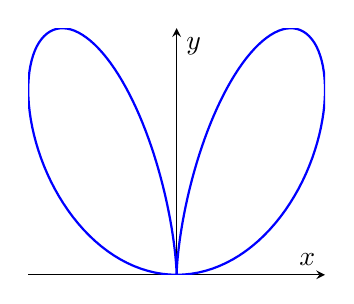
\begin{tikzpicture}
  \begin{axis}[
    ytick=\empty,
    xtick=\empty,
    scale=0.55,
    axis lines=middle,
    xlabel={$x$},
    ylabel={$y$},
  ]
    \addplot [
      domain=0:pi,
      samples=200,
      thick,
      blue,
      data cs=polarrad,
    ] {cos(deg(x))*cos(deg(x))*sin(deg(x))};
  \end{axis}
\end{tikzpicture}
\end{minipage}

\item Find the projection of the point $P(1,2,3)$ onto the plane $x+y+z=0$.
\begin{center}
\begin{tabular}{lllll}
(A) $(-1,0,1)$ &
(B) $(1,1,-2)$ &
(C) $(0,0,0)$ &
(D) $(-1,-1,2)$ &
(E) $(1,2,-3)$
\end{tabular}
\end{center}

\item Find the area of the region inside the circle $r=3\cos\theta$ and outside the cardioid $r=1+\cos\theta$.
\begin{center}
\begin{tabular}{lllll}
(A) $\pi$ &
(B) $\pi/2$ &
(C) $2\pi$ &
(D) $3\pi/4$ &
(E) $1$
\end{tabular}
\end{center}

\item Identify the quadric surface defined by the equation $2z^2 - x^2/2 - y^2 - 5 = 0$.
\begin{center}
\begin{tabular}{ll}
(A) Hyperboloid of two sheets &
(B) Hyperboloid of one sheet 
\end{tabular}

\begin{tabular}{lll}
(C) Elliptic paraboloid &
(D) Cone &
(E) Cylinder
\end{tabular}
\end{center}

\item In which direction does $f(x,y,z) = x^2 + 2y^2 - 3z$ increase most rapidly at $P(1,1,2)$?
\begin{center}
\begin{tabular}{lllll}
(A) $\langle 2, 4, -3 \rangle$ &
(B) $\langle 1, 1, -3 \rangle$ &
(C) $\langle -2, -4, 3 \rangle$ &
(D) $\langle 2, 4, 0 \rangle$ &
(E) $\langle 1, 2, -3 \rangle$
\end{tabular}
\end{center}

\item Let $w = \ln(x^2 + y^2)$ where $x = s\cos t$ and $y = s + \sin t$. Find $\dfrac{\partial w}{\partial t}$ at $(s,t) = (1, \pi/6)$.
\begin{center}
\begin{tabular}{lllll}
(A) $0$ &
(B) $1$ &
(C) $3/2$ &
(D) $\sqrt{3}/2$ &
(E) $\sqrt{3}/3$ 
\end{tabular}
\end{center}

\item Find the arc length of the curve $y = x^2/2, z = x^3/6$ from $x = 0$ to $x = 2$.
\begin{center}
\begin{tabular}{lllll}
(A) $10/3$ &
(B) $8/3$ &
(C) $4$ &
(D) $7/3$ &
(E) $3$
\end{tabular}
\end{center}

\newpage
\item A vector parallel to the tangent line of the intersection of $z = x^2 + 2y^2$ and $x^2 + (y-1)^2 = 1$ at $P(1,1,3)$ is:
\begin{center}
\begin{tabular}{lllll}
(A) $\langle 0, 2, 8 \rangle$ &
(B) $\langle 2, 4, -1 \rangle$ &
(C) $\langle 2, 0, 0 \rangle$ &
(D) $\langle 1, 1, 3 \rangle$ &
(E) $\langle 4, -2, -8 \rangle$
\end{tabular}
\end{center}

\item Which is a valid parametrization for the intersection of $z = x^2 + y^2$ and $z = 4$?
\begin{center}
\begin{tabular}{ll}
(A) $\vec{r}(t) = \langle 2\cos t, 2\sin t, 4 \rangle$ &
(B) $\vec{r}(t) = \langle \cos t, \sin t, 4 \rangle$
\end{tabular}

\begin{tabular}{lll}
(C) $\vec{r}(t) = \langle 2\cos t, 2\sin t, t \rangle$ &
(D) $\vec{r}(t) = \langle t, t^2, 4 \rangle$ &
(E) $\vec{r}(t) = \langle 2\cos t, 2\sin t, 2 \rangle$
\end{tabular}
\end{center}

\item Consider the system of equations:
\[
\begin{cases}
xu^2v + y\cos(u) = 1 \\
\ln(uv) + x^2y - u + v = 0
\end{cases}
\]
Assume that this system defines $u$ and $v$ implicitly as functions of $x$ and $y$ near the point $P(x,y,u,v) = (1,0,1,1)$.
Show that the system can be solved for $u$ and $v$ in terms of $x$ and $y$ near $P$ and find the value of $\partial u / \partial y$ at $P$.

\item \begin{enumerate}[label=\textbf{\alph*.}]
\item Consider the function
\[f(x,y) = \begin{cases}
\frac{x^2 + \sin(x)\cos(y)}{x}, & x \neq 0 \\ 
1, & x = 0 
\end{cases}.\]
Find $f_x(0,0)$ using the formal definition of the partial derivative.
    
\item Evaluate the following limit or show that it does not exist.
\[\lim_{(x,y)\to(0,0)} \frac{x^3 y^2}{x^6 + y^4}\]
\end{enumerate}

\item Find the absolute maximum and minimum values of the function
\[f(x,y) = x^2 + y^2 - 2x + 4y\]
on the closed triangular region $D$ with vertices $(0,0)$, $(4,0)$, and $(0,-4)$. Show all your work, including the analysis of the interior critical points and the boundary of the region.
\end{enumerate}

\newpage
\pagestyle{fancy}
\renewcommand{\headrulewidth}{1pt}
\fancyhead[R]{\textit{2025-2026 Spring Midterm}}
\fancyhead[L]{\textit{Hacettepe MAT124 Exam Solutions Version 2}}

%Last update: 05/09/2026 01:59

\begin{enumerate}[leftmargin=*,label=\textbf{\arabic*.}]

\item Given cylindrical coordinates $(r, \theta, z) = \left(\sqrt{3}, -\frac{\pi}{4}, -1\right)$. Using conversion formulas:
\begin{align*}
\rho &= \sqrt{r^2 + z^2} = \sqrt{(\sqrt{3})^2 + (-1)^2} = \sqrt{3 + 1} = 2 \\
\theta &= -\frac{\pi}{4} \\
\phi &= \arccos\left(\frac{z}{\rho}\right) = \arccos\left(-\frac{1}{2}\right) = \frac{2\pi}{3}
\end{align*}

Thus $(\rho, \theta, \phi) = \left(2, -\frac{\pi}{4}, \frac{2\pi}{3}\right)$.

$\boxed{\text{Answer: (A)}}$

\item We can solve this question by trial and error. Inspect $r = \cos^2\theta \sin\theta$.
\begin{itemize}[leftmargin=*]
    \item When $\theta = 0, \pi$, $r = 0$.
    \item For $\theta \in (0, \pi)$, $\sin\theta > 0$ and $\cos^2\theta \ge 0$, creating a loop along the positive $y$-axis.
    \item The factor $\cos^2\theta$ pinches the loop at $\theta = \frac{\pi}{2}$, matching the given shape.
\end{itemize}

$\boxed{\text{Answer: (A)}}$

\item Given point $P(1,2,3)$ and plane $x + y + z = 0$ with normal vector $\vec{n} = \langle 1, 1, 1 \rangle$.

The orthogonal line through $P$ is $\vec{r}(t) = \langle 1+t, 2+t, 3+t \rangle$. Substitute into the plane equation.
\[(1+t) + (2+t) + (3+t) = 0 \implies 3t + 6 = 0 \implies t = -2\]

Substitute $t = -2$ back yields the projection point.
\[P' = (1 - 2, 2 - 2, 3 - 2) = (-1, 0, 1)\]

$\boxed{\text{Answer: (A)}}$

\item Find intersection points for $r_1 = 3\cos\theta$ and $r_2 = 1 + \cos\theta$.
\[3\cos\theta = 1 + \cos\theta \implies 2\cos\theta = 1 \implies \theta = \pm \frac{\pi}{3}\]

Calculate area.
\begin{align*}
    A &= \frac{1}{2} \int_{-\pi/3}^{\pi/3} \left( r_1^2 - r_2^2 \right) d\theta = \int_{0}^{\pi/3} \left( 8\cos^2\theta - 2\cos\theta - 1 \right) d\theta \\
      &= \int_{0}^{\pi/3} \left( 3 + 4\cos 2\theta - 2\cos\theta \right) d\theta \\
      &= \left[ 3\theta + 2\sin 2\theta - 2\sin\theta \right]_0^{\pi/3} = \pi
\end{align*}

$\boxed{\text{Answer: (A)}}$

\item Rearrange $2z^2 - \frac{x^2}{2} - y^2 - 5 = 0$.
\[\frac{z^2}{5/2} - \frac{x^2}{10} - \frac{y^2}{5} = 1\]

The standard form $\frac{z^2}{c^2} - \frac{x^2}{a^2} - \frac{y^2}{b^2} = 1$ has two negative minus signs and one positive sign, representing a hyperboloid of two sheets.

$\boxed{\text{Answer: (A)}}$

\item The direction of maximum increase of $f(x,y,z) = x^2 + 2y^2 - 3z$ is given by gradient $\nabla f$:
\[\nabla f = \langle 2x, 4y, -3 \rangle\]

Evaluate at $P(1,1,2)$.
\[\nabla f(1,1,2) = \langle 2, 4, -3 \rangle\]

$\boxed{\text{Answer: (A)}}$

\item Given $w = \ln(x^2 + y^2)$, $x = s\cos t$, and $y = s + \sin t$. At $(s,t) = \left(1, \frac{\pi}{6}\right)$:
\[x = \frac{\sqrt{3}}{2}, \quad y = \frac{3}{2}, \quad x^2 + y^2 = 3\]

Applying the Chain Rule $\frac{\partial w}{\partial t} = \frac{\partial w}{\partial x}\frac{\partial x}{\partial t} + \frac{\partial w}{\partial y}\frac{\partial y}{\partial t}$:
\begin{align*}
    \frac{\partial w}{\partial x} &= \frac{2x}{x^2+y^2} = \frac{\sqrt{3}}{3}, \quad &\frac{\partial x}{\partial t} &= -s\sin t = -\frac{1}{2} \\
    \frac{\partial w}{\partial y} &= \frac{2y}{x^2+y^2} = 1, \quad &\frac{\partial y}{\partial t} &= \cos t = \frac{\sqrt{3}}{2}
\end{align*}
\[\frac{\partial w}{\partial t} = \left(\frac{\sqrt{3}}{3}\right)\left(-\frac{1}{2}\right) + (1)\left(\frac{\sqrt{3}}{2}\right) = \frac{\sqrt{3}}{3}\]

$\boxed{\text{Answer: (E)}}$

\item For $y = \frac{x^2}{2}$ and $z = \frac{x^3}{6}$, derivatives are $\frac{dy}{dx} = x$ and $\frac{dz}{dx} = \frac{x^2}{2}$.
\begin{align*}
    L &= \int_{0}^{2} \sqrt{1 + \left(\frac{dy}{dx}\right)^2 + \left(\frac{dz}{dx}\right)^2} \, dx = \int_{0}^{2} \sqrt{1 + x^2 + \frac{x^4}{4}} \, dx \\
      &= \int_{0}^{2} \left(1 + \frac{x^2}{2}\right) dx = \left[ x + \frac{x^3}{6} \right]_{0}^{2} = \frac{10}{3}
\end{align*}

$\boxed{\text{Answer: (A)}}$

\item For $F(x,y,z) = x^2 + 2y^2 - z = 0$ and $G(x,y,z) = x^2 + (y-1)^2 - 1 = 0$, gradients at $P(1,1,3)$ are:
\[\nabla F(1,1,3)=\langle 2, 4, -1 \rangle, \quad \nabla G(1,1,3) = \langle 2, 0, 0 \rangle\]

Cross product gives the tangent vector.
\[\vec{v} = \nabla F \times \nabla G = \begin{vmatrix} \mathbf{i} & \mathbf{j} & \mathbf{k} \\ 2 & 4 & -1 \\ 2 & 0 & 0 \end{vmatrix} = \langle 0, -2, -8 \rangle\]

Negating yields the parallel vector $\langle 0, 2, 8 \rangle$.

$\boxed{\text{Answer: (A)}}$

\item Intersecting $z = x^2 + y^2$ and $z = 4$ gives $x^2 + y^2 = 4$ in the plane $z = 4$.

Standard parametrization is
\[\vec{r}(t)=\langle2\cos t,2\sin t,4\rangle\]

$\boxed{\text{Answer: (A)}}$

\item Jacobian matrix with respect to $(u,v)$ at $P(1,0,1,1)$:
\[J = \begin{bmatrix} \frac{\partial x}{\partial u} & \frac{\partial x}{\partial v} \\[1em] \frac{\partial y}{\partial u} & \frac{\partial y}{\partial v} \end{bmatrix}_{\text{at } P}  = \begin{bmatrix} 2xuv - y\sin u & xu^2 \\ \frac{1}{u} - 1 & \frac{1}{v} + 1 \end{bmatrix}_{\text{at } P} = \begin{bmatrix} 2 & 1 \\ 0 & 2 \end{bmatrix}\]

Since $\det(J)=2\cdot2-1\cdot0=4\neq0$, the system defines $u, v$ implicitly near $P$. Differentiate with respect to $y$.
\begin{align*}
    2u \frac{\partial u}{\partial y} + \frac{\partial v}{\partial y} + \cos(1) &= 0 \implies 2\frac{\partial u}{\partial y} + \frac{\partial v}{\partial y} = -\cos(1) \\
    2\frac{\partial v}{\partial y} + 1 &= 0 \implies \frac{\partial v}{\partial y} = -\frac{1}{2}
\end{align*}

Substitute $\frac{\partial v}{\partial y}$.

\[\boxed{\frac{\partial u}{\partial y} = \frac{1 - 2\cos(1)}{4}}\]

\item \begin{enumerate}[label=\textbf{\alph*.}]
    \item Use the formal definition of $f_x(0,0)$.
    \[f_x(0,0) = \lim_{h \to 0} \frac{f(h,0) - f(0,0)}{h} = \lim_{h \to 0} \frac{\frac{h^2 + \sin(h)}{h} - 1}{h} = \lim_{h \to 0} \frac{h^2 + \sin(h) - h}{h^2}\]
    Use L'Hôpital's rule twice.
    \[f_x(0,0) \overset{\text{L'H.}}= \lim_{h\to0}\frac{2h+\cos h-1}{2h}\overset{\text{L'H.}}= \lim_{h\to0}\frac{2-\sin h}{2}=\frac{2-0}2=\boxed1\]
    \item Approach $\displaystyle\lim_{(x,y)\to(0,0)} \frac{x^3 y^2}{x^6 + y^4}$ along paths $y = k x^{3/2}$.
    \[\lim_{x \to 0^+} \frac{x^3 (k^2 x^3)}{x^6 + k^4 x^6} = \frac{k^2}{1 + k^4}\]
    Since the result depends on $k$, $\boxed{\text{the limit does not exist}}$.
\end{enumerate}

\item The extreme value theorem states that a continuous function on a specific region will always have its absolute maxima and minima. $f$ is continuous everywhere on its domain. Check the interior points.
\[\nabla f = \langle 2x - 2, 2y + 4 \rangle = \langle 0, 0 \rangle \implies (1, -2)\]

Check if the point is inside the region.
\[y > x -4\longrightarrow 1 - (-2) = 3 < 4\]

$(1,-2)$ is inside. We have $f(1,-2) = -5$.

Check the boundary.
\begin{itemize}[leftmargin=*]
    \item $x=0$: $g(y) = y^2 + 4y \implies y = -2 \implies f(0,-2) = -4$
    \item $y=0$: $h(x) = x^2 - 2x \implies x = 1 \implies f(1,0) = -1$
    \item $y = x - 4$: $k(x) = 2x^2 - 6x \implies x = \frac{3}{2},\: y = -\frac{5}{2} \implies f\left(\frac{3}{2}, -\frac{5}{2}\right) = -4.5$
\end{itemize}

Check the endpoints. At endpoints: $f(0,0) = 0$, $f(0,-4) = 0$, and $f(4,0) = 8$.

Compare all the values obtained.

\[\boxed{\text{Absolute minimum value is }{-5}\text{ at }(1,-2).\text{ Absolute maximum value is }8\text{ at }(4,0).}\]

\end{enumerate}
\end{document}